\chapter{The Truck Backer-Upper}
% Authors: Xiao Jing, Arnav Kansal, Changgeng Zhao, 4/30/19.

\section{Set up}
We try to design a self-learning nonlinear controller to control the steering of a trailer truck while backing up a loading dock from an arbitrary initial position. Only backing up is allowed to park the truck parallel to the dock and trying to match ($x_{trailer}$, $y_{trailer}$) with ($x_{dock}$, $y_{dock}$) as closely as possible. In the lecture, some students tried to play this game and we found it's very hard even for humans to accomplish the task.
\\
\begin{figure}[H]
    \centering
    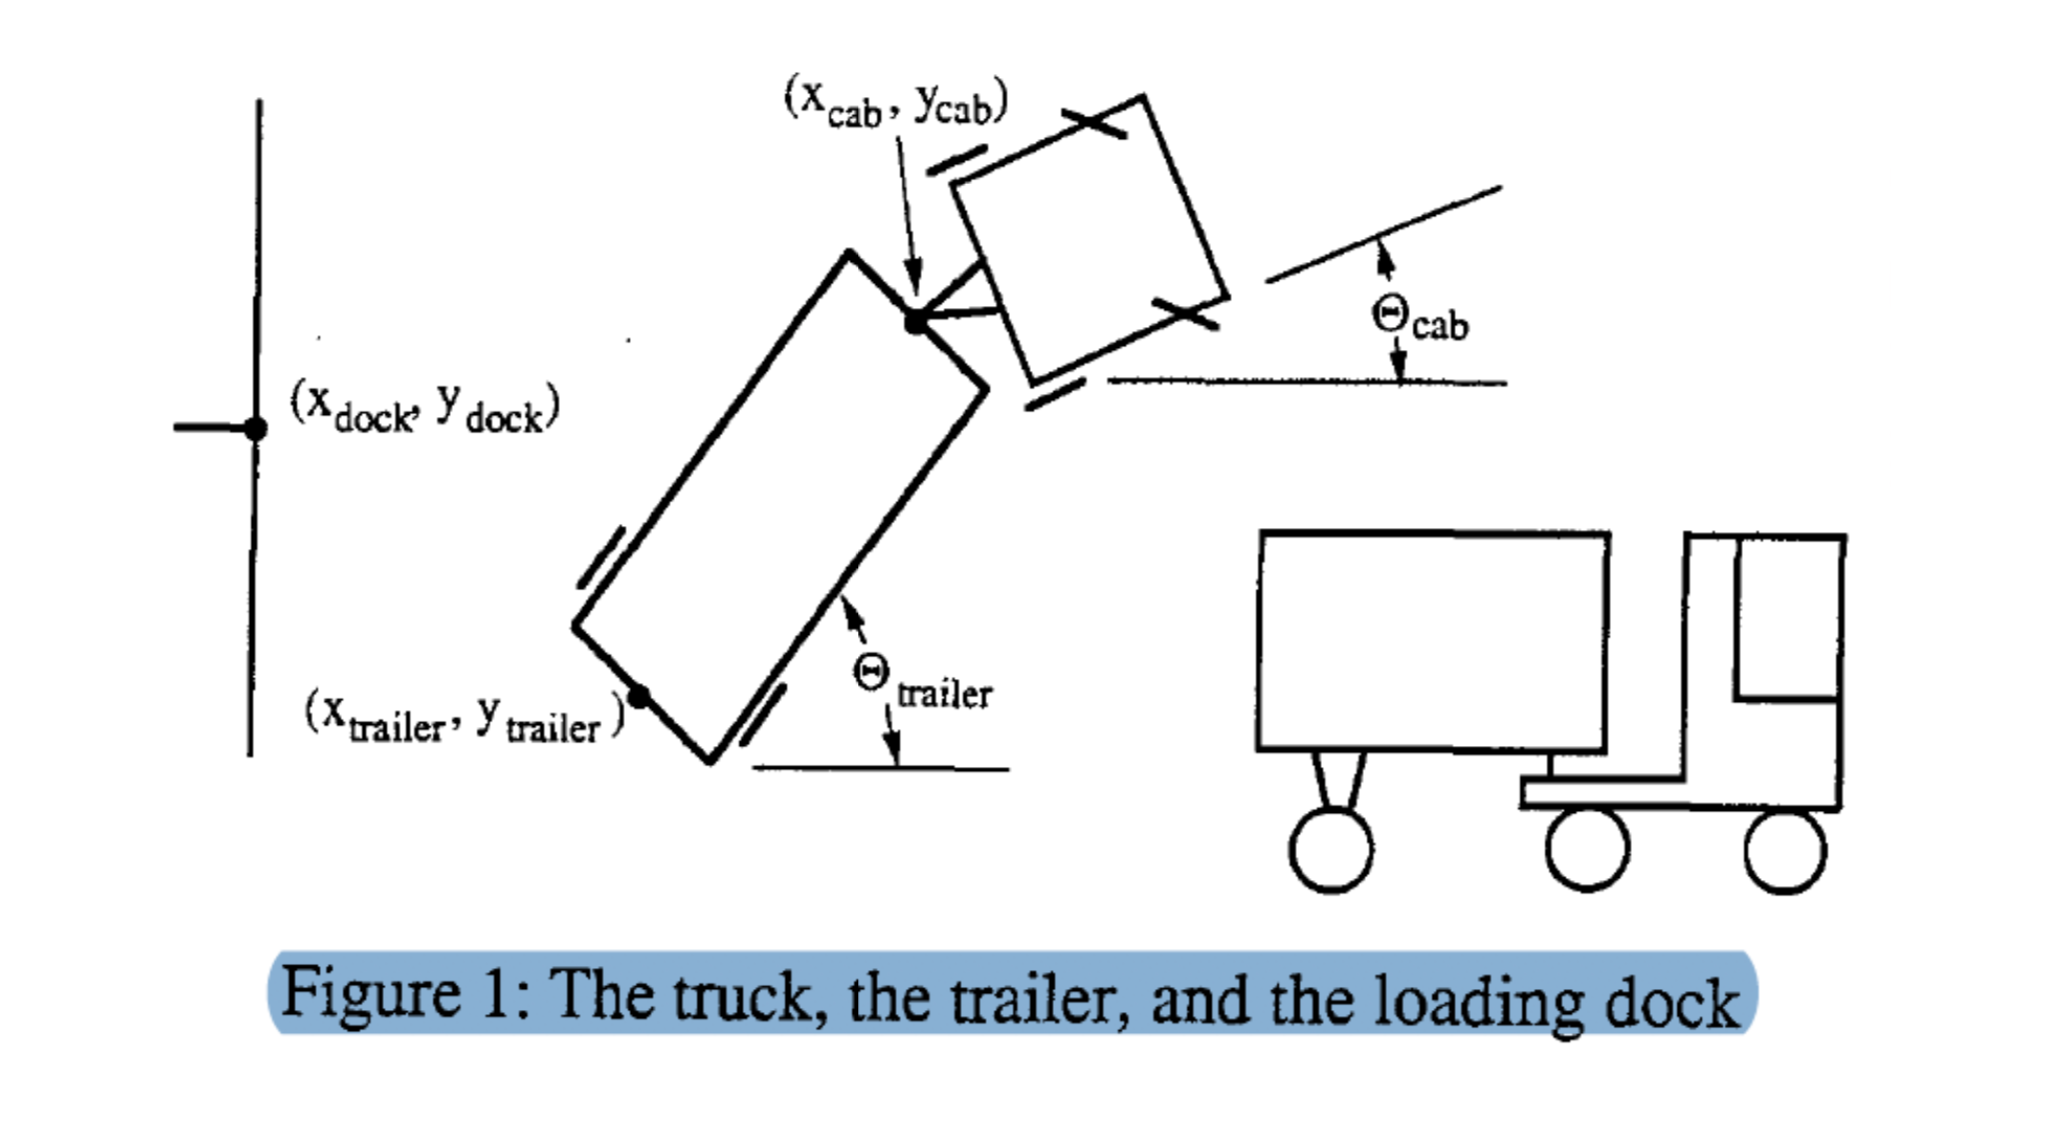
\includegraphics[width=0.7\textwidth]{figs/figure1.png}
    \caption{The Truck, trailer and loading dock}
    \label{fig:general}
\end{figure}
State variables representing the position of the truck: $\theta_{cab}$, the angle of the truck, $x_{cab}$ and $y_{cab}$, the cartesian position of the yoke, $x_{trailer}$ and $y_{trailer}$, the cartesian position of the rear of the center of the trailer, $\theta_{trailer}$, the angle of the trailer.

\section{Model and two stage learning}
\subsection{Model}
\begin{figure}[H]
    \centering
    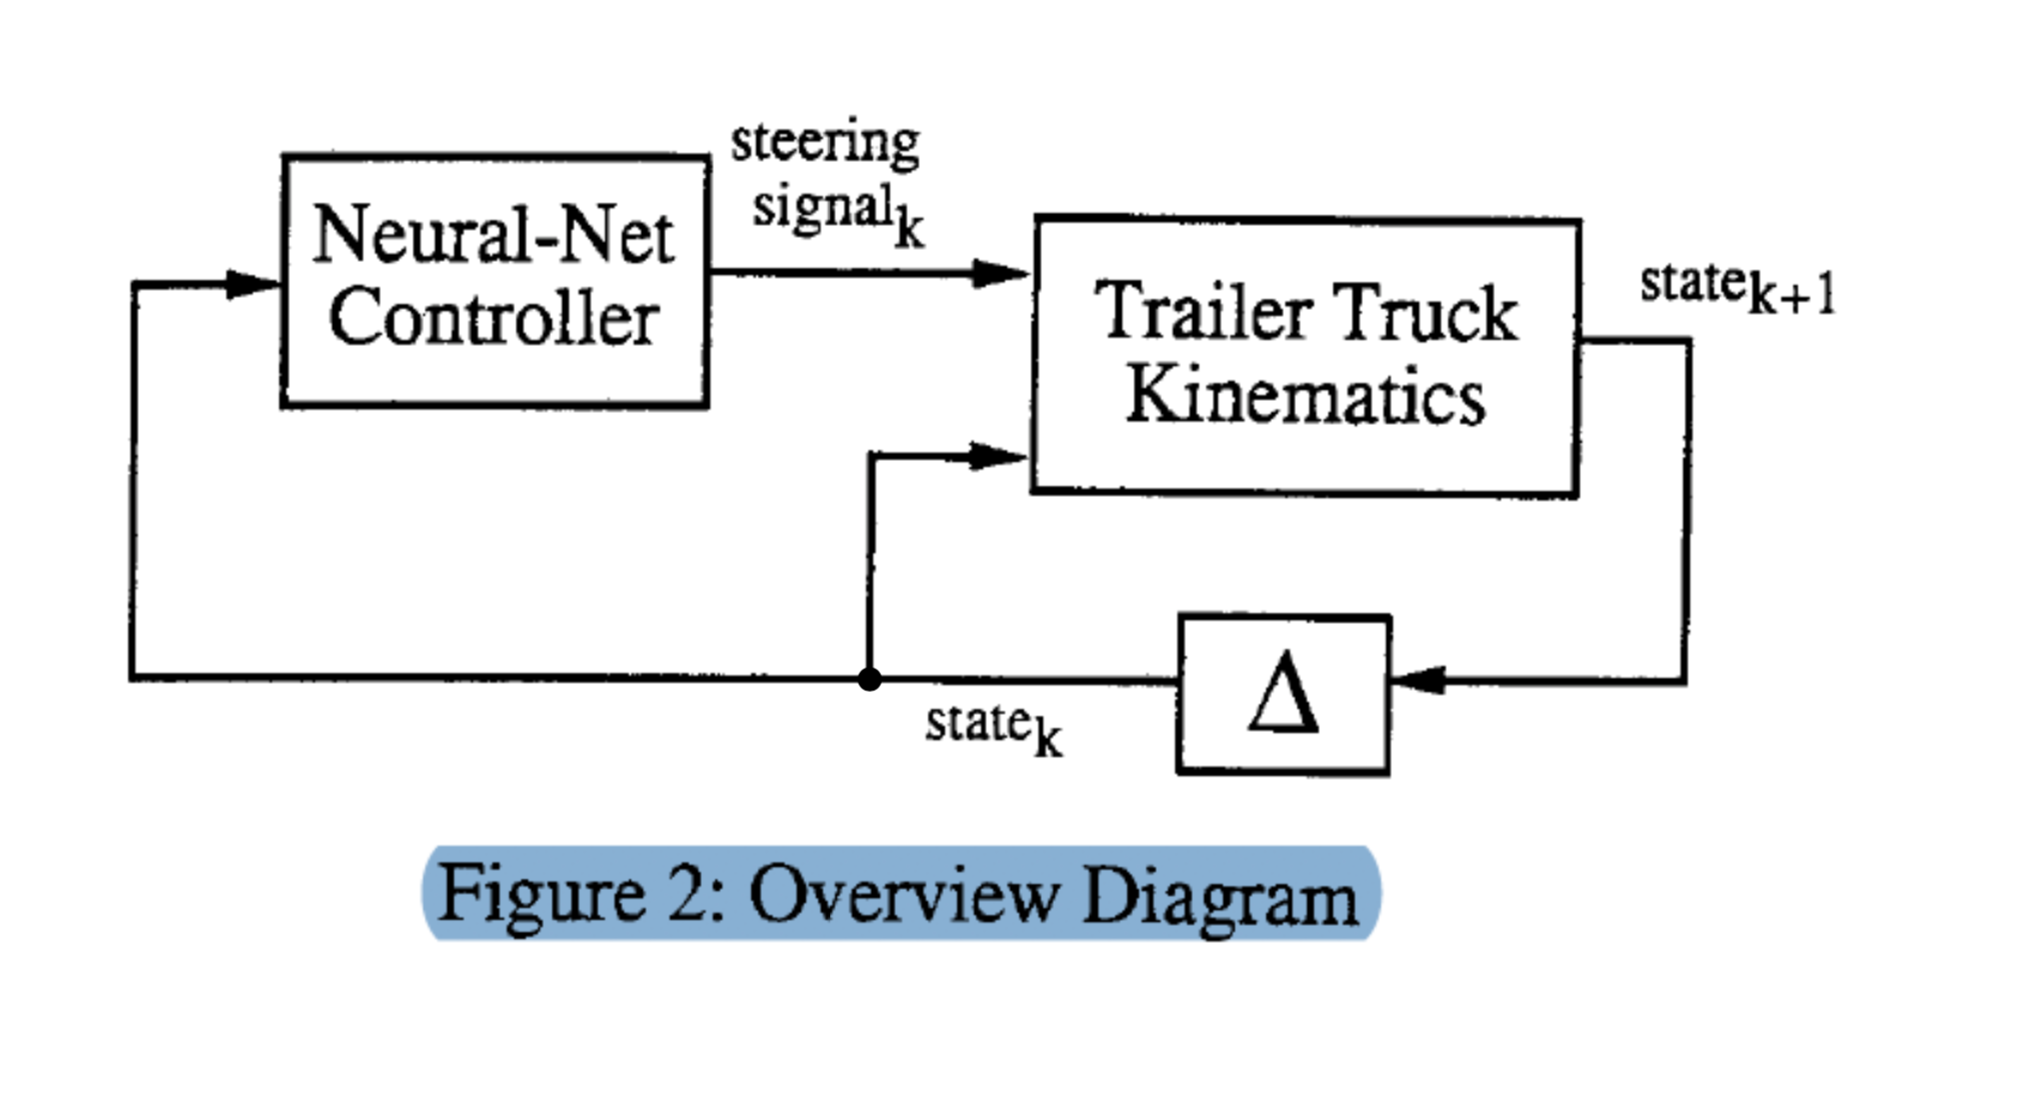
\includegraphics[width=0.6\textwidth]{figs/figure2.png}
    \caption{The two part model}
    \label{fig:learn}
\end{figure}
The proposed model has two elements: the \textbf{Kinematics Component} (emulator) and the \textbf{Neural Net Controller}. The trailer truck Kinematics Component of the model tries to learn the next state of the truck given the current state and the steering action. The Neural Net Controller learns the steering action given the current state of the truck. We train the two models separately: first train the Kinematics Component and then based on this model we train the Controller by back-prop through Kinematics model.


 
\subsection{Variable Input}
In the paper, there are 6 parameters. However, we just need 4 variables in state $k$, which are shown in the next slide, since cab coordinate can be calculated according to the four values we have.
\begin{figure}[H]
    \centering
    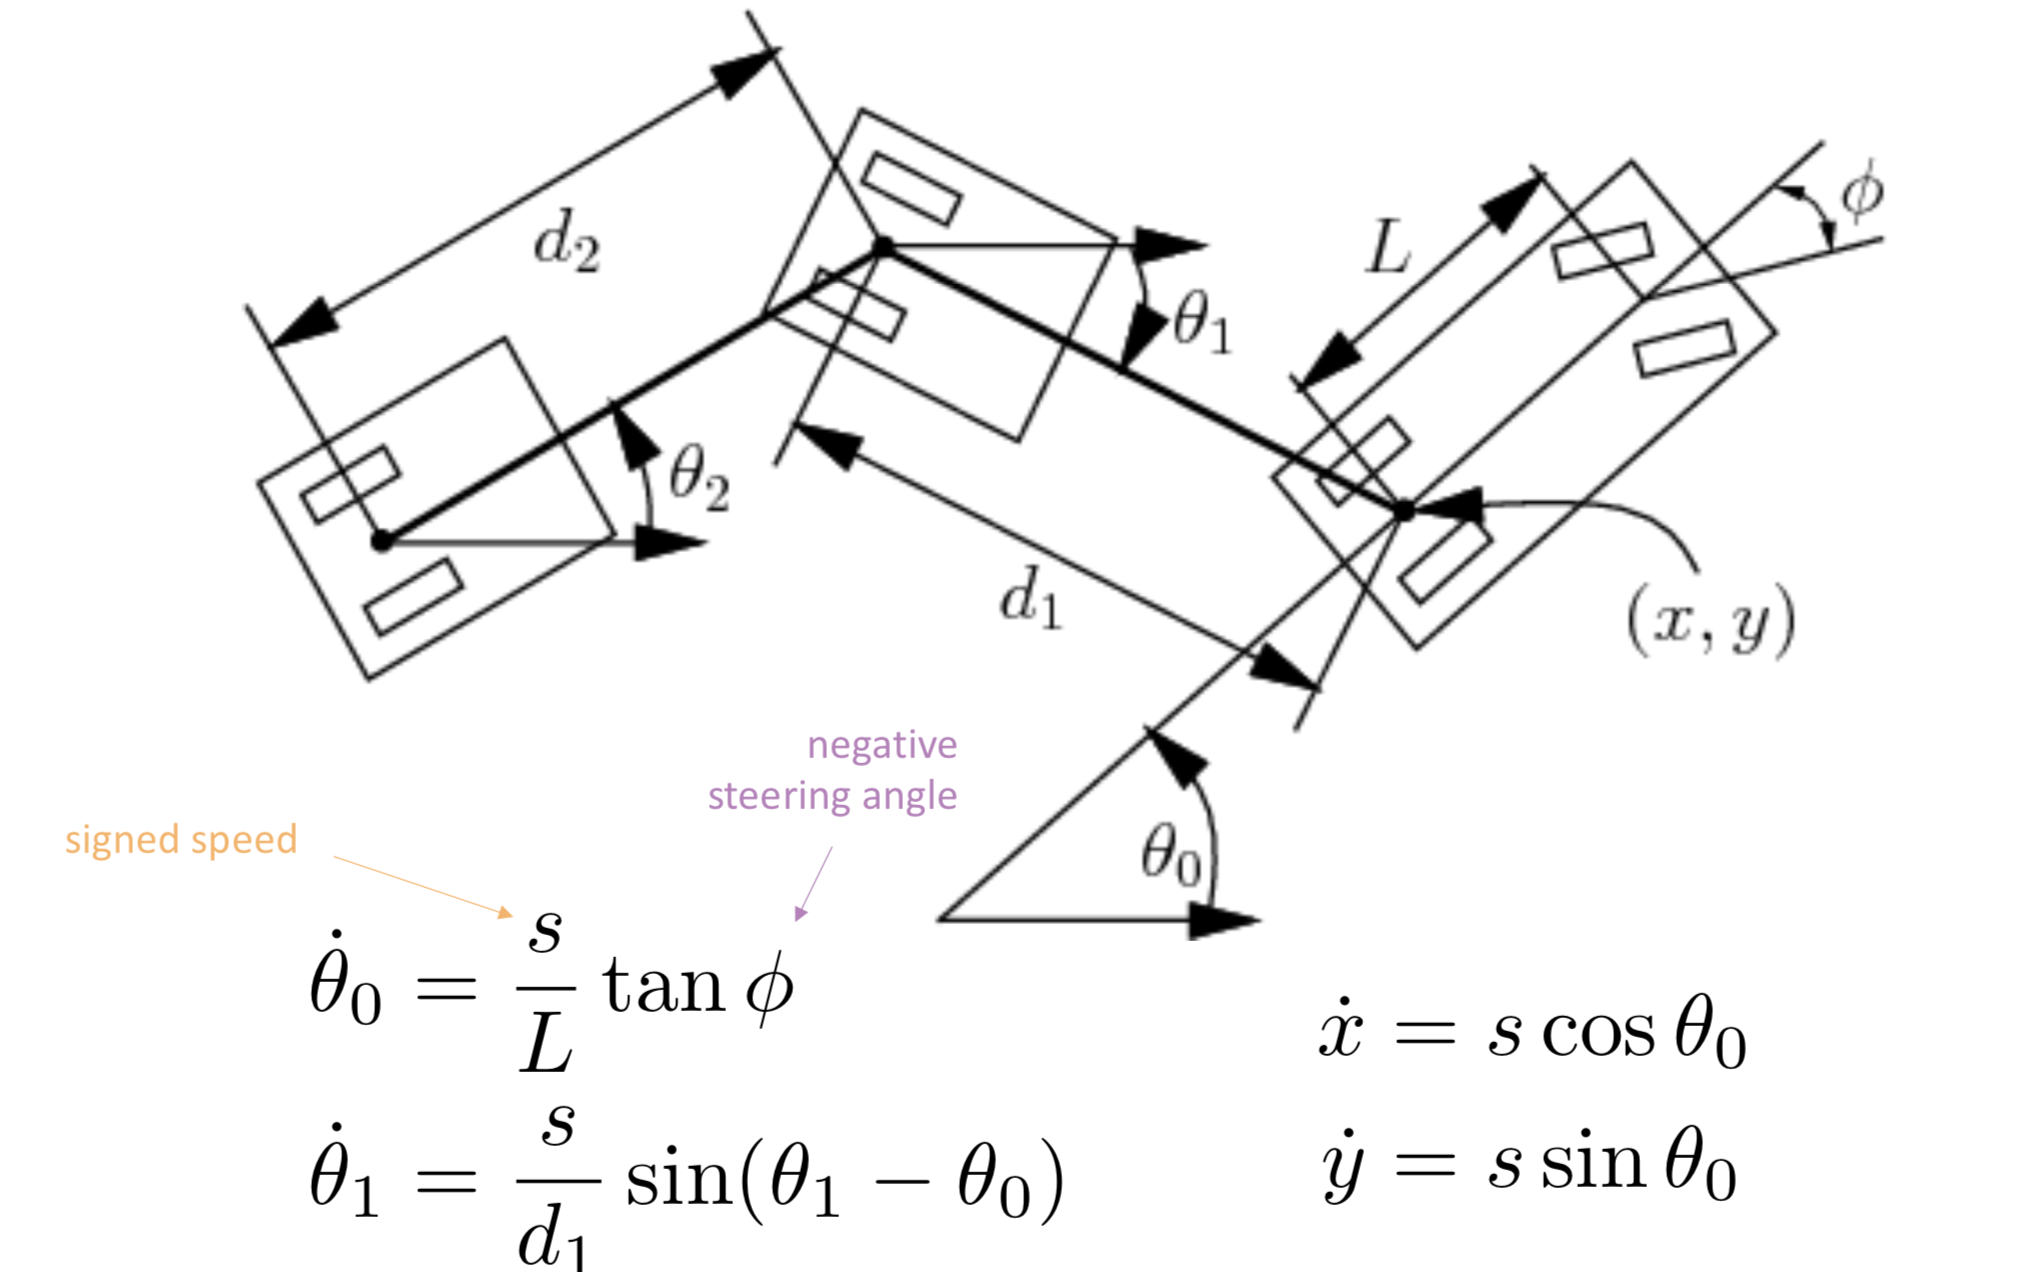
\includegraphics[width=0.6\textwidth]{figs/variable.png}
    \caption{Variable}
    \label{fig:variable}
\end{figure}

\subsection{Flow chart}
The block labeled $C$ represent the controller and $T$ represent the emulator. The initial position of truck is chosen at random. The final error is used by back-propagation to adapt to each state Controller/Trailer.
\begin{figure}[H]
    \centering
    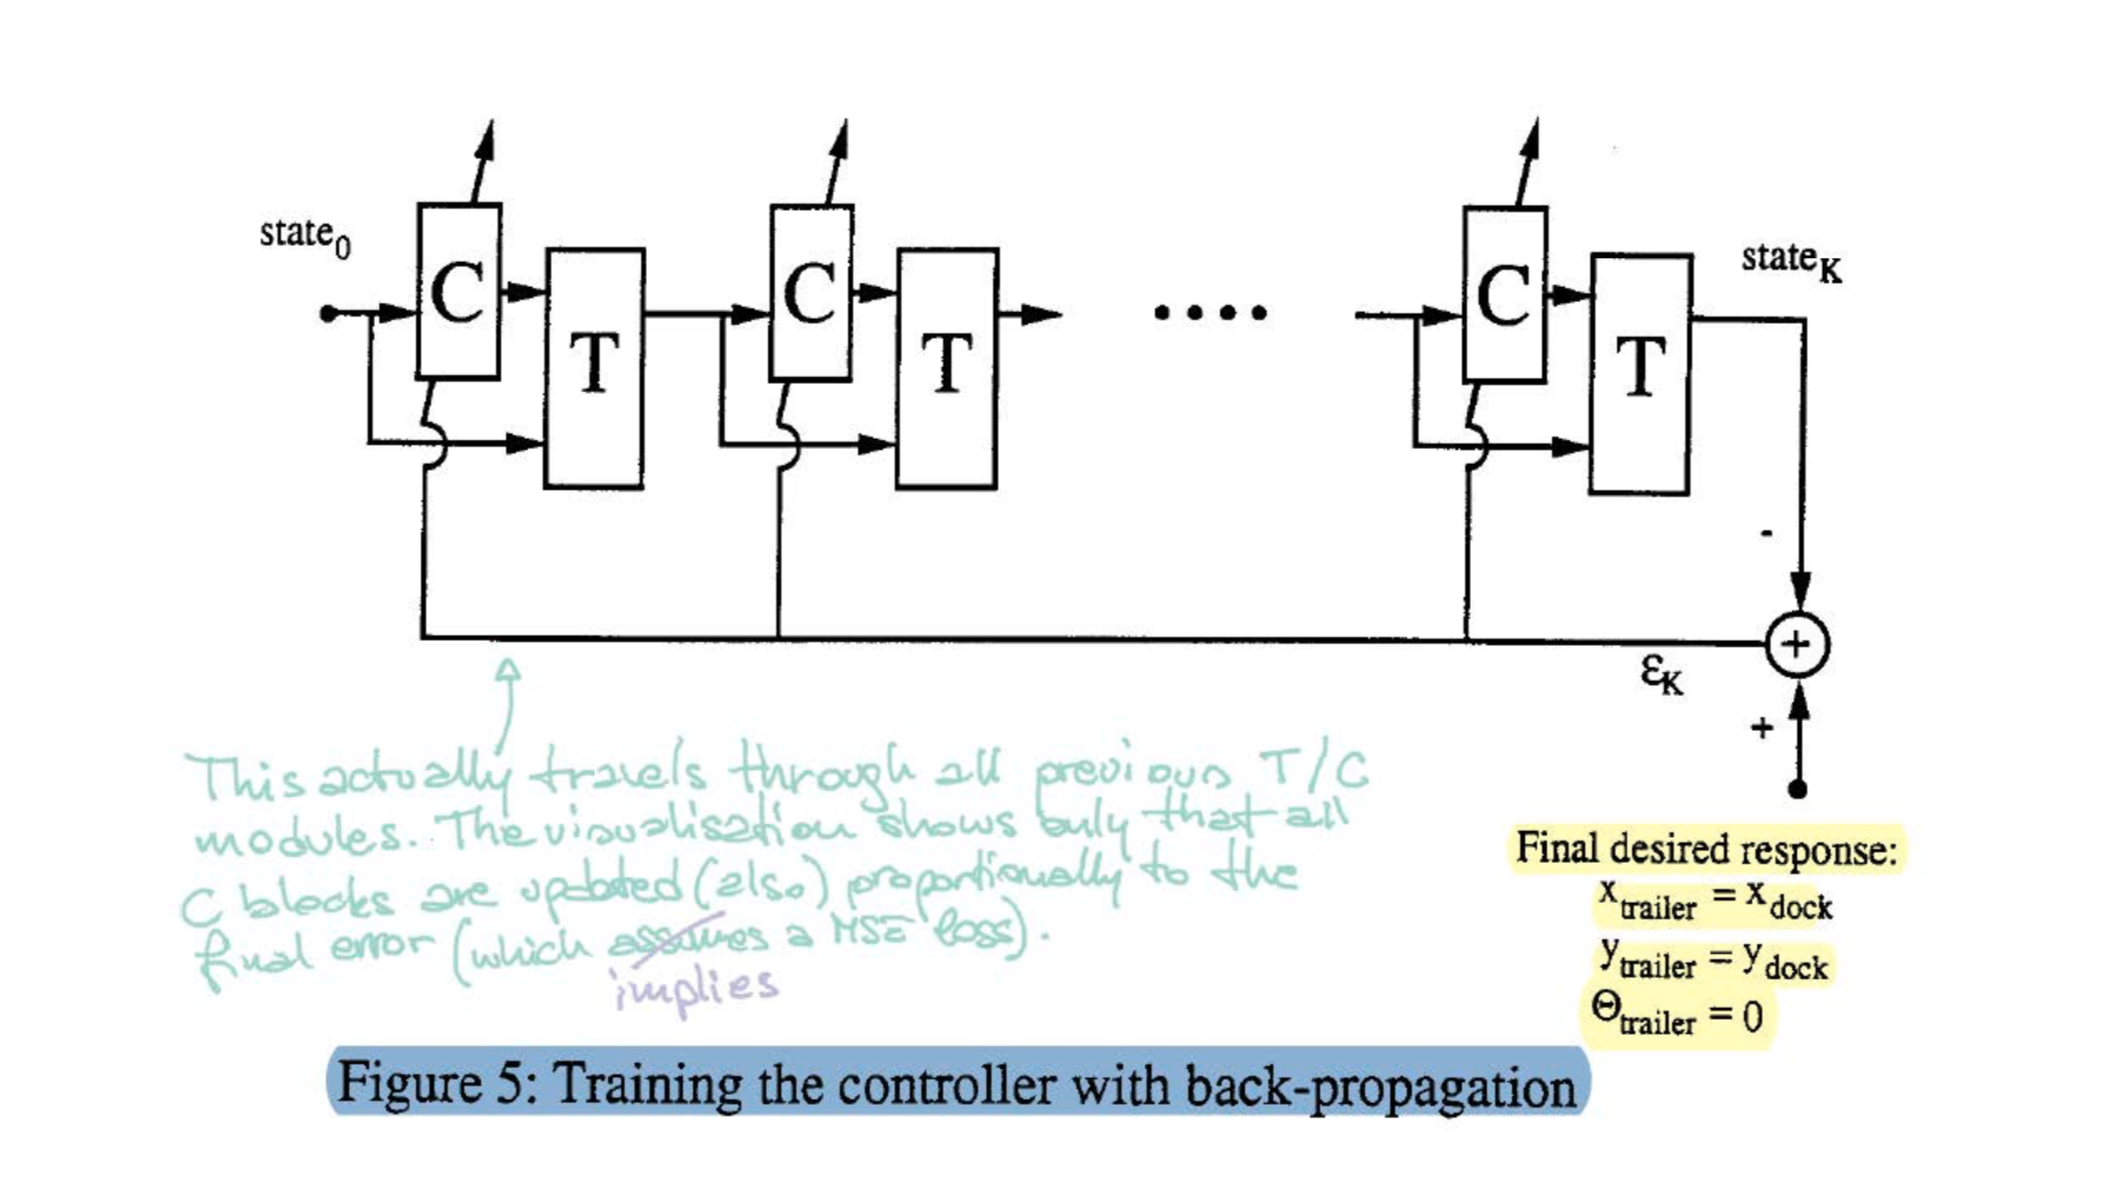
\includegraphics[width=0.8\textwidth]{figs/figure5.png}
    \label{fig:loss}
\end{figure}
Each time, we have 6 inputs for controller at state $k$, and we add bias and forward the inputs to 25 hidden units, and give 1 output unit. So there are 3 layers in the controller. 
\\
Then we put the controller's output to the Emulator, which has 45 hidden units and 6 output for the next state. It is analogous to a neural network having a number of layers equal to four times the number of backing up steps.
\begin{figure}[H]
    \centering
    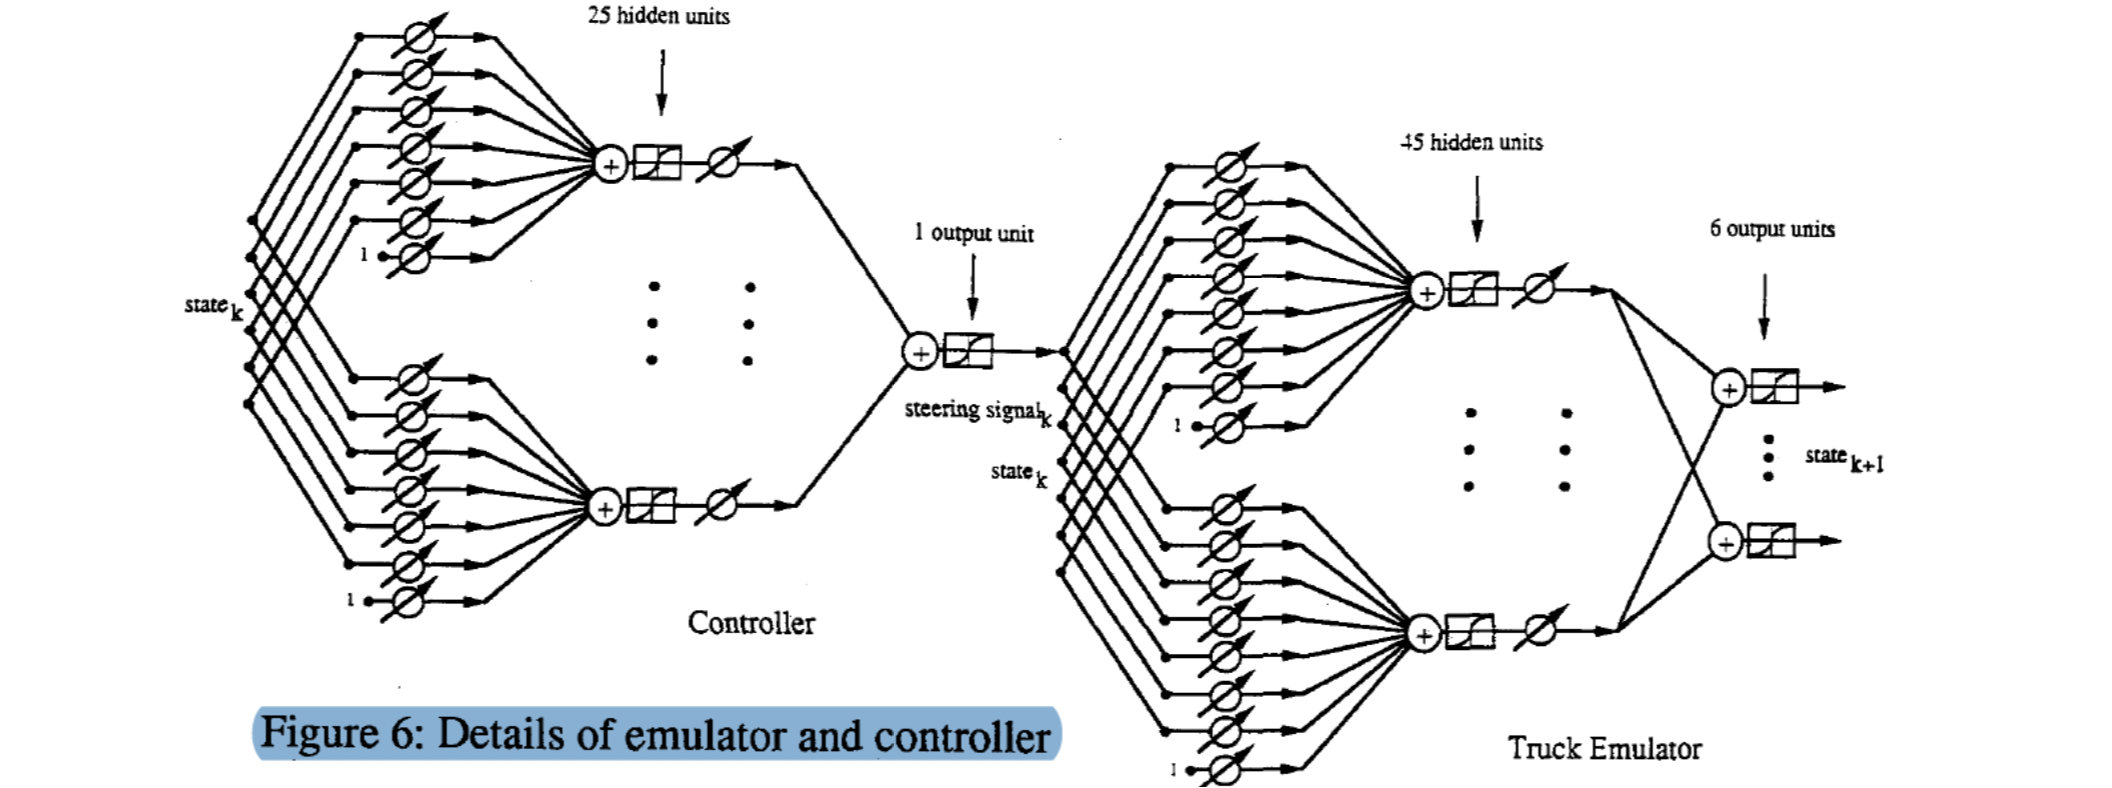
\includegraphics[width=0.8\textwidth]{figs/figure6.png}
    \label{fig:nn}
\end{figure}

\subsection{Loss Function}
Here the $\theta_c$ is $\theta_0$, the $\theta_t$ is $\theta_1$

\begin{equation*}
    ||\theta_{t}||^2 + ||(x_{\text{trailer}}, y_{\text{trailer}}) - (x_{\text{dock}}, y_{\text{dock}})||^2     
\end{equation*}

% \begin{figure}[H]
%     \centering
%     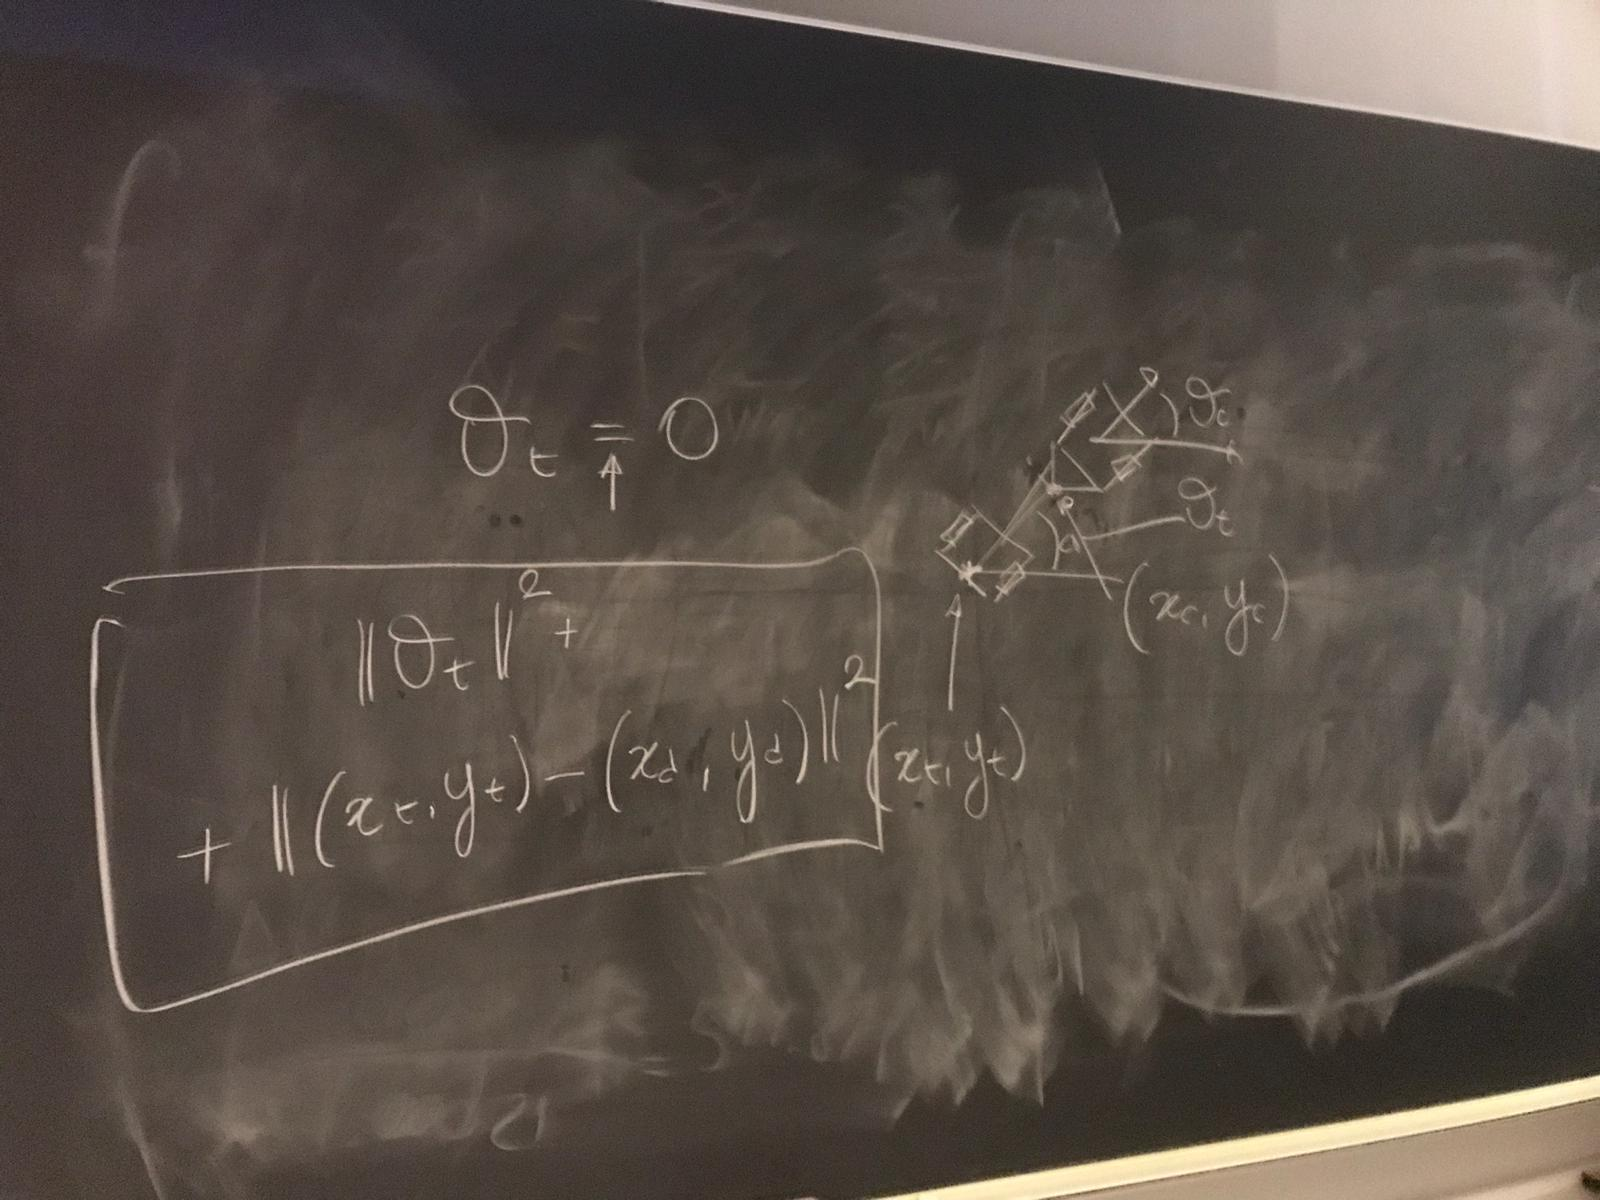
\includegraphics[width=0.7\textwidth]{labs/13/images/loss.jpeg}
%     \caption{loss}
%     \label{fig:loss}
% \end{figure}



\subsection{Two stage Learning}\label{sec:truck-model}
In the first stage of learning, the emulator is fed as input : states of the truck along with random steering actions and the actual state of the truck (according to the physics of the system) as output to learn. The emulator can then predict the next state of the truck given an initial state and the steering action.

The second stage of learning involves unrolling the controller for the length of the actions of the episode and recursively applying the controller to the states produced by the action the controller takes. This produces a final state of the truck which is used to calculate the loss and used to update the parameters of the controller via back propagation through time.

\begin{itemize}
\item Q: Why don't we use the kinematics equations directly as we already know how a track move? 
-- A: Because we want to show that the model can learn the kinematics facts automatically, which is useful in other complicated scenarios where we can not know how it works.
\end{itemize}

\subsection{Initial to final state}
Traces of trajectory guided by the learned system in action.
\begin{figure}[H]
    \centering
    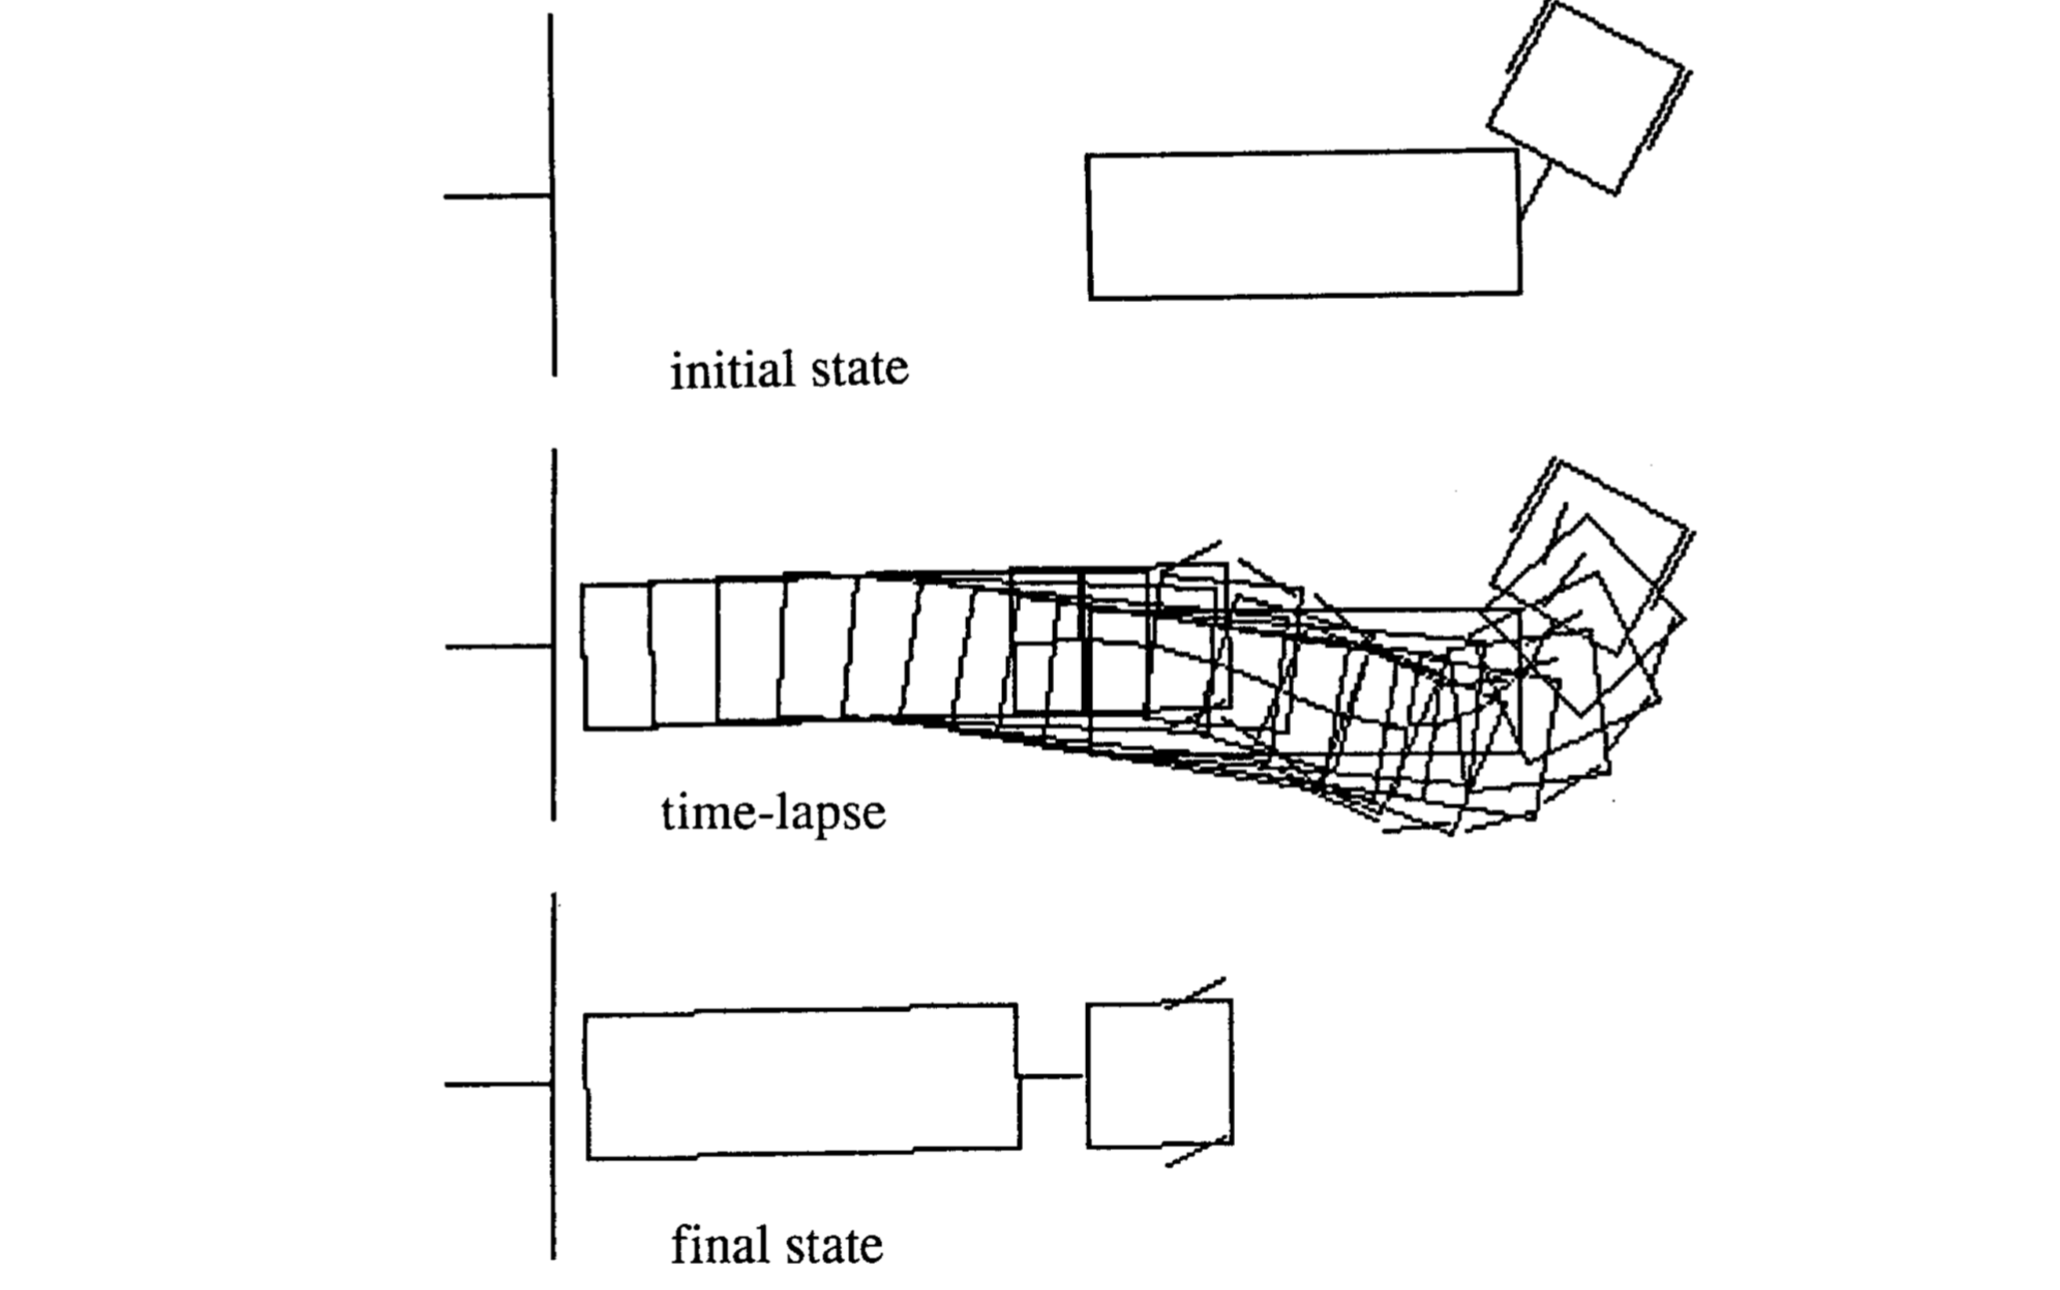
\includegraphics[width=0.45\textwidth]{figs/state.png}
    \label{fig:state}
    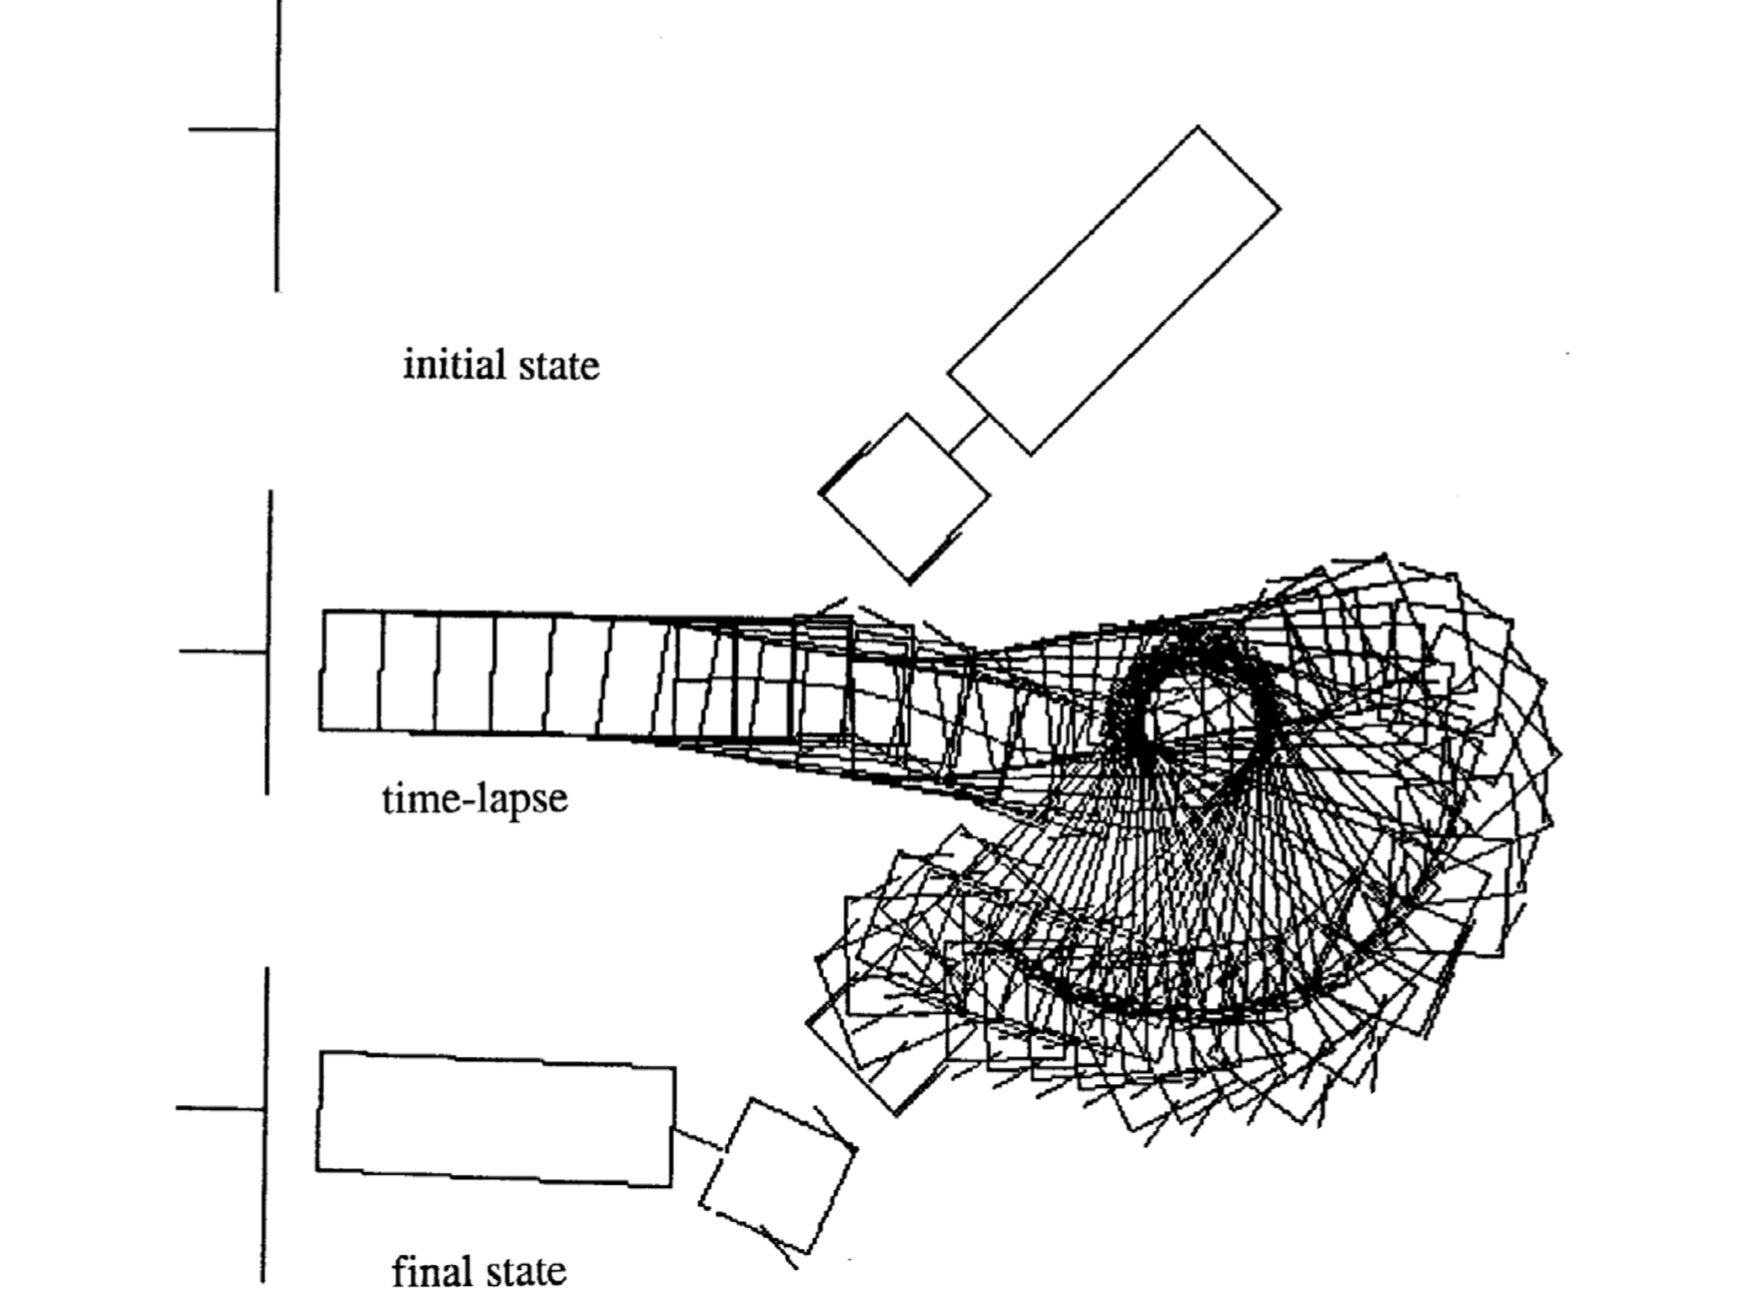
\includegraphics[width=0.45\textwidth]{figs/state2.png}
    \label{fig:state2}
\end{figure}